\documentclass[
  12pt,				    % tamanho da fonte
  openright,			% capítulos começam em pág ímpar (insere página vazia caso preciso)
  oneside,			    % para impressão em recto e verso. Oposto a oneside
  a4paper,			    % tamanho do papel. 
  chapter=TITLE,        % títulos de capítulos convertidos em letras maiúsculas
  section=TITLE,        % títulos de seções convertidos em letras maiúsculas
  english,			    % idioma adicional para hifenização
  french,			    % idioma adicional para hifenização
  spanish,			    % idioma adicional para hifenização
  brazil				% o último idioma é o principal do documento
]{iftex}

% ------------------------------------------------------------------------------- %
% DADOS BASE DO TCC                                                               %
% ------------------------------------------------------------------------------- %
\autor{Nome do aluno}


% ======= TITULOS  =========
\titulo{Titulo do TCC}

\instituicao{Instituto}
\curso{Curso}
\local{Cidade}
\data{Ano}
% ------------------------------------------------------------------------------- %
\tipotrabalho{Trabalho de Conclusão de Curso}
\preambulo{Preambulo do Trabalho}

\orientador[Orientador][Prof. Dr.]{Fulano}[De tal]{Instituto Federal do Espírito Santo - Cachoeiro de Itapemirim}
% \coorientador[Coorientadora][Profa. Dra.]{Beltrana}[de Tal]{Instituto Federal do Espírito Santo}

\examinadori{Dra. Fulana de Tal}{Instituto Federal do Espírito Santo - Cachoeiro de Itapemirim}{Examinadora}
\examinadorii{Dr. Cicrano de Tal}{Instituto Federal do Espírito Santo  - Cachoeiro de Itapemirim}{Examinador}

\approvaldate{21}{Fevereiro}{2022}


% ------------------------------------------------------------------------------- %
% PALAVRAS CHAVES                                                                 %
% ------------------------------------------------------------------------------- %
\palavraschave{Palavra 1}[Palavra 2][Palavra 3][Palavra 4][OPalavra 5]
\keywords{word 1}[word 2][word 3][word 4][word 5]


% ------------------------------------------------------------------------------- %
% FICHA CATALOGRÁFICA                                                             %
% ------------------------------------------------------------------------------- %
\fichabiblioteca{
    % Dados Internacionais de Catalogação-na-Publicação (CIP) \\
    (Biblioteca Carlos Drummond de Andrade do Instituto Federal do Espírito Santo)
}
\fichaautor{Elaborada por Aluno – CRB-X/ES - XXX}
\fichatags{
    1. Palavra 1.  2. Palavra 2. 3. Palavra 3. 4. Palavra 4. 5. Palavra 5 I. Nome Orientador II. Instituto. III. Título.
}

\cutter{X999y}
\cdd{000.00}
\selectlanguage{brazil}



% ------------------------------------------------------------------------------- %
% FONT                                                                            %
% ------------------------------------------------------------------------------- %
%(para usar times-new-roman, comente as três linhas abaixo)
\usepackage{helvet}
\renewcommand{\familydefault}{\sfdefault}
\renewcommand{\ABNTEXchapterfont}{\bfseries}


% ------------------------------------------------------------------------------- %
% ELEMENTOS OPCIONAIS                                                             %
% ------------------------------------------------------------------------------- %
\editardedicatoria{%---------------------------------
%      FOLHA DE DEDICATÓRIA
%---------------------------------

Texto aqui!
}
\editaragradecimentos{%---------------------------------
%     FOLHA DE AGREDECIMENTO
%---------------------------------

Texto aqui!}
\editarepigrafe{%---------------------------------
%       FOLHA DE EPIGRAFE
%---------------------------------

\textbf``O cosmos é tudo o que existe, que existiu ou que existirá."\\Carl Sagan}

% ------------------------------------------------------------------------------- %
% LISTAS [siglas e Símbolos]                                                      %
% ------------------------------------------------------------------------------- %
\editarlistasiglas{%---------------------------------
%        LISTA DE SIGLAS
%---------------------------------

\begin{siglas}
    \item [AEB] Agência Espacial Brasileira
    \item [GDD] Game Design Document
    \item [OBA] Olimpíada Brasileira de Astronomia e Astronáutica
\end{siglas}}
\editarlistasimbolos{%---------------------------------
%       LISTA DE SIMBOLOS
%---------------------------------

\begin{simbolos}
    \item[$\lambda$] Letra grega labda
\end{simbolos}}

\newcommand{\ie}{\textit{i.e. }}
\newcommand{\eg}{\textit{e.g. }}


\begin{document}

    % ======= ELEMENTOS-PRÉ-TEXTUAIS =========
    \capas                                  % 
    \imprimircapa                           % 
    \imprimirfolhaderosto                   % 
    \imprimirfichacatalografica             % 
    
    \pretextual
    \imprimiraprovacao                      % 
    \imprimirdeclaracao                     % 
    \imprimirdedicatoria                    % 
    \imprimiragradecimentos                 % 
    \imprimirepigrafe                       % 
    
    %---------------------------------
%       FOLHA DE RESUMO
%---------------------------------

\begin{resumo}
    \vspace{-15pt}
    
    Texto aqui!


    Palavras-chave: \palavraschaveemlinha
\end{resumo}


%---------------------------------
%       FOLHA DE ABSTRACT
%---------------------------------

\begin{resumo}[Abstract]
    \vspace{-15pt}
    
    \begin{otherlanguage*}{english}
    
        Texto aqui!
        
        Keywords: \inlinekeywords
    \end{otherlanguage*}
\end{resumo}             % 
    
    % ================ LISTAS ================ 
    \imprimirlistafiguras                   % 
    \imprimirlistatabelas                   % 
    \imprimirlistaquadros                   % 
    \imprimirlistasiglas                    % 
    \imprimirlistasimbolos                  % 

    \imprimirsumario                        % 
    
    % ========= ELEMENTOS-TEXTUAIS ===========
    \textual
    \graphicspath{{figuras/}}   
     %---------------------------------
%           INTRODUÇÃO
%---------------------------------


\chapter[Introdução]{Introdução}
\vspace{1cm}

Texto Aqui!


% ========= JUSTIFICATIVA =========
\section{Justificativa}

Texto Aqui!



% ========= OBJETIVOS =========
\section{Objetivos}

\subsection{Geral}

Texto Aqui!

\subsection{Específicos}
\begin{itemize}
	\item Item 01;
	
	\item Item 02;
    
    \item Item 03;
    
    \item Item 04;
\end{itemize}



% ========= ESTR. TRABALHO =========
\section{Estrutura do trabalho}

Este trabalho será didaticamente dividido em capítulos, de forma a facilitar a compreensão do leitor, sendo estes expostos a seguir:

\begin{itemize}
    \item Capítulo 1: Introdução - ;

    \item Capítulo 2: Referencial Teórico - ;
    
    \item Capítulo 3: Materiais e Métodos - ;
    
    \item Capítulo 4: Resultado e Discussões - ;
    
    \item Capítulo 5: Considerações Finais - ;

\end{itemize}             % 
    %---------------------------------
%       REFERENCIAL TEÓRICO
%---------------------------------

\chapter[Referencial Teórico]{Referencial Teórico}


\section{Citação}

Citação 01 - ``Lorem Ipsum is simply dummy text of the printing and typesetting industry. Lorem Ipsum has been the'' \cite{AEB:20} \\\\
Citação 02 - Segundo \citeonline{Machado:11}, Lorem Ipsum is simply dummy text of the printing and typesetting industry.\\

\begin{citacao}
   Lorem Ipsum is simply dummy text of the printing and typesetting industry. Lorem Ipsum has been the industry's standard dummy text ever since the 1500s, when an unknown printer took a galley of type and scrambled it to make a type specimen book. It has survived. \cite{Sagan:19}
\end{citacao}

\begin{itemize}
    \item item 01;
    \item item 02;
    \item item 03.
\end{itemize}


\section{Figura}

\begin{figure}[ht]
    \caption{Contextualização da gamificação}
    \label{fig:game}
    \centering
    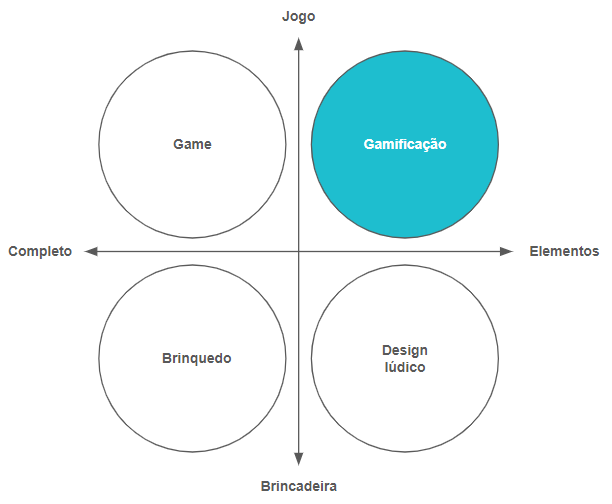
\includegraphics[width=0.5\textwidth]{figuras/Gamificação.png}
    \legend{Elaboração Própria}
\end{figure}


\section{Tabela}

\begin{table}[ht]
  \caption{Comparativo entre ferramentas similares}
  \label{Tab: Comparativo EA}
  \centering
  
  \begin{tabularx}{\textwidth}{p{4.4cm} ccccc}
    \hline
    \footnotesize\bfseries{Software} & \footnotesize\bfseries{Astronomia}   & \footnotesize\bfseries{Astronáutica}  & \footnotesize\bfseries{Mobile}  & \footnotesize\bfseries{Gamificação} & \footnotesize\bfseries{Português}\\
    \hline
    
        \footnotesize{Astronomia}              & x &   & x & x & x \\
        \footnotesize{Astronomy}               & x &   & x &   &   \\
        \footnotesize{Curso de Astronomia}     & x &   & x &   & x \\
        \footnotesize{ESApp}                   & x & x & x &   & x \\
        \footnotesize{Nasa}                    & x & x & x &   & x \\
        \footnotesize{Pockocmoc}               & x & x & x &   &   \\
        \footnotesize{Space Launch Now}        &   & x & x &   & x \\
        \footnotesize{Spacetoday}              & x & x &   &   & x \\
        \footnotesize{Stellarium}              & x &   & x &   & x \\
        \footnotesize{Space Learn}             & x & x & x & x & x \\ 
   
    \hline
  \end{tabularx}

  \legend{Elaboração Própria}
\end{table}

\section{Quadro}

\begin{quadro}[ht]
    \caption{Estrutura do GDD}
    \label{quad:gdd}
    \centering
    \begin{tabular}{|ll|}
        \cline{1-2}
        I.      & Resumo do Jogo            \\
        II.     & Descrição do Jogo         \\
        III.    & Informações Básica        \\
        IV.     & Planejamento Interno      \\
        V.      & Análises                  \\
        VI.     & Gameplay                  \\
        VII.    & Níveis                    \\
        VIII.   & Controle de versão        \\
        IX.     & Cronograma                \\
        \cline{1-2}
    \end{tabular}
    
    \legend{Elaboração Própria}
\end{quadro}

\vspace{2cm}

\section{Tabela grande}
\begin{table}[ht]
    \caption{Critérios da Técnica de Thomas Reeves}
    \label{Tab: CriterioThomas}
    \centering
    
    \begin{tabularx}{\textwidth}{m{.4cm} m{5cm} l}
        
        \hline
        \multicolumn{2}{c}{\footnotesize\bfseries{Critérios}} & \multicolumn{1}{c}{\footnotesize\bfseries{Conceitos}}\\
        \hline
        
        \multirow{14}{*}{\footnotesize\rotatebox{90}{Critérios Pedagógicos}}
        & \footnotesize{1. Epistemologia}                                 & \footnotesize{Objetivista              $\longleftrightarrow$ Construtivista}                  \\
        & \footnotesize{2. Filosofia Pedagógica}                          & \footnotesize{Instrutivista            $\longleftrightarrow$ Construtivista}                  \\
        & \footnotesize{3. Psicologia Subjacente}                         & \footnotesize{Comportamental           $\longleftrightarrow$ Cognitiva}                       \\
        & \footnotesize{4. Objetividade}                                  & \footnotesize{Precisamente Focalizado  $\longleftrightarrow$ N-Focalizado}                    \\
        & \footnotesize{5. Sequenciamento Instrucional}                   & \footnotesize{Reducionista             $\longleftrightarrow$ Construtivista}                  \\
        & \footnotesize{6. Validade Experimental}                         & \footnotesize{Abstrato                 $\longleftrightarrow$ Concreto}                        \\
        & \footnotesize{7. Papel Instrutor}                               & \footnotesize{Provedor de Materiais    $\longleftrightarrow$ Agente}                          \\
        & \footnotesize{8. Valoriazação do Erro}                          & \footnotesize{Aprendizado sem Erro     $\longleftrightarrow$ Aprendizado com a experiência}   \\
        & \footnotesize{9. Motivação}                                     & \footnotesize{Extrínseca               $\longleftrightarrow$ Intrínseca}                      \\
        & \footnotesize{10. Estruturação}                                 & \footnotesize{Alta                     $\longleftrightarrow$ Baixa}                           \\
        & \footnotesize{11. Diferenças individuais}                       & \footnotesize{Não existente            $\longleftrightarrow$ Multi-facetada}                  \\
        & \footnotesize{12. Controle do Aluno}                            & \footnotesize{Não existente            $\longleftrightarrow$ Irrestrito}                      \\
        & \footnotesize{13. Atividade do Usuário}                         & \footnotesize{Matemagênico             $\longleftrightarrow$ Generativo}                      \\
        & \footnotesize{14. Aprendizado Cooperativo}                      & \footnotesize{Não suportado            $\longleftrightarrow$ Integral}                        \\
    
        \hline
        
        \multirow{10}{*}{\footnotesize\rotatebox{90}{Critérios de Interface}}
        & \footnotesize{15. Facilidade de Uso}                            & \footnotesize{Difícil                  $\longleftrightarrow$ Fácil}                           \\
        & \footnotesize{16. Navegação}                                    & \footnotesize{Difícil                  $\longleftrightarrow$ Fácil}                           \\
        & \footnotesize{17. Carga Cognitiva}                              & \footnotesize{Não                      $\longleftrightarrow$ Gerenciável / Intuitiva}         \\
        & \footnotesize{18. Mapeamento}                                   & \footnotesize{Nenhum                   $\longleftrightarrow$ Poderoso}                        \\
        & \footnotesize{19. Design de Tela}                               & \footnotesize{Princípios violados      $\longleftrightarrow$ Princípios respeitados}          \\
        & \footnotesize{20. Simetria do Conhecimento}                     & \footnotesize{Incompatível             $\longleftrightarrow$ Compatível}                      \\
        & \footnotesize{21. Apresentação da Informação}                   & \footnotesize{Confusa                  $\longleftrightarrow$ Clara}                           \\
        & \footnotesize{22. Integração das Mídias}                        & \footnotesize{Não Coordenada           $\longleftrightarrow$ Coordenada}                      \\
        & \footnotesize{23. Estética}                                     & \footnotesize{Desagradável             $\longleftrightarrow$ Agradável}                       \\
        & \footnotesize{24. Funcionalidade Geral}                         & \footnotesize{Não funciona             $\longleftrightarrow$ Altamente funcional}             \\
        
        \hline
    \end{tabularx}
    
    \legend{Adaptado de \citeonline{Cybis:00}}
\end{table}

\clearpage

% https://www.seer.ufrgs.br/index.php/renote/article/view/53496/33013
% \footnotemark
% \footnotetext {Disponível em: <>. Acesso em: xx ______ xxxx.}
            % 
    %---------------------------------
%       MATERIAIS E MÉTODOS
%---------------------------------

\chapter[Materiais e Métodos]{Materiais e Métodos}

Texto Aqui!            % 
    %---------------------------------
%    RESULTADOS E DISCUSSÕES
%---------------------------------

\chapter[Resultados e Discussões]{Resultados e Discussões}

Texto Aqui!             % 
    %---------------------------------
%       CONSIDERAÇÕES FINAIS
%---------------------------------

\chapter[Considerações finais]{Considerações finais}

Texto Aqui!          % 
    
    % ======= ELEMENTOS-PÓS-TEXTUAIS =========
    \postextual
    
    \bibliographystyle{abntex2-alf}
    \bibliography{bibliografia}
    
    % % Apêndices
    % \begin{apendicesenv}
    %     \chapter{{\normalfont Explicação}}
\label{apendice: a}

É um elemento opcional. É um documento elaborado pelo próprio autor com o objetivo de completar sua argumentação, sem que haja prejuízo para a unidade do trabalho (ASSOCIAÇÃO BRASILEIRA DE NORMAS TÉCNICAS, 2011b. Deve ser precedido da palavra APÊNDICE (ex:APÊNDICE A, APÊNDICE B), identificado por letras maiúsculas consecutivas, travessão e pelo respectivo título. 
    % \end{apendicesenv}
    
    % Índice Remissivo
    \phantompart
    \printindex

\end{document}